\documentclass[10pt, final]{article}
% \documentclass[10pt,technote]{IEEEtran}
\usepackage[a4paper,width=185mm,top=20mm,bottom=20mm]{geometry}
\usepackage{pythonhighlight}
\usepackage{url}
\usepackage{lipsum}
\usepackage{amsmath, amssymb}
\usepackage{multicol}
\setlength{\columnsep}{1cm}
\usepackage{graphicx}
\graphicspath{{../results/}{../immagini/}}
\DeclareGraphicsExtensions{.png, .pdf}
\usepackage{wrapfig}
\usepackage[font=small,labelfont=bf]{caption}
\usepackage{setspace}
\usepackage{caption}
\usepackage{subcaption}
\usepackage{wrapfig}
\usepackage{float}
\usepackage{xcolor}
\usepackage[tikz]{mdframed}
\usepackage{colortbl}
\usepackage{MnSymbol}
\usepackage[utf8]{inputenc}
\usepackage[T1]{fontenc}
\usepackage{ascii}
\usepackage{listings}

\lstset{prebreak=\raisebox{0ex}[0ex][0ex]
        {\ensuremath{\rhookswarrow}}}
\lstset{postbreak=\raisebox{0ex}[0ex][0ex]
        {\ensuremath{\rcurvearrowse\space}}}
\lstset{breaklines=true, breakatwhitespace=true}
\lstset{numbers=left, numberstyle=\scriptsize}
\DeclareMathOperator{\E}{\mathbb{E}}

\UseRawInputEncoding %%%%%%%%%%%%%%%%%%%%%%%%%OCCHIOOOOOO
\definecolor{forestgreen}{rgb}{0.0, 0.27, 0.13}
%%
%% Julia definition (c) 2014 Jubobs
%%
\lstdefinelanguage{Julia}%
  {morekeywords={abstract,break,case,catch,const,continue,do,else,elseif,%
      end,export,false,for,function,immutable,import,importall,if,in,%
      macro,module,otherwise,quote,return,switch,true,try,type,typealias,%
      using,while},%
   sensitive=true,%
   alsoother={\$},%
   morecomment=[l]\#,%
   morecomment=[n]{\#=}{=\#},%
   morestring=[s]{"}{"},%
   morestring=[m]{'}{'},%
}[keywords,comments,strings]%

\lstset{%
    language         = Julia,
    basicstyle       = \ttfamily,
    keywordstyle     = \bfseries\color{blue},
    stringstyle      = \color{magenta},
    commentstyle     = \color{forestgreen},
    showstringspaces = false,
}


\definecolor{airforceblue}{rgb}{0.36, 0.54, 0.66}
\mdfsetup{
middlelinecolor=airforceblue,%
middlelinewidth=0.2pt,%
roundcorner=5pt}
\setlength{\abovedisplayskip}{3pt}
\setlength{\belowdisplayskip}{3pt}

\renewcommand{\baselinestretch}{1}

\title{\textsc{Report 2 - Grangier-Roger-Aspect experiment analysis}}
\author{Francesco Lorenzi,      October 2020}
\date{}
\begin{document}
\maketitle
\vspace{-25pt}

\begin{center}
	\rule[0pt]{400pt}{0.5pt}
\end{center}
\vspace{-15pt}

\begin{multicols}{2}
\subsubsection*{Summary}
The purpose of this report is twofold: in a first part a statistical analysis will be carried out on a dataset collected from an experimental setup based on Grangier-Roger-Aspect experiment \cite{grangier}. 

In a second part, an application of photon arrival statistics is shown: using a dataset from coherent light photon detection, random integers are generated and analyzed using various visual techniques.

\section{Photon indivisibility experiment}
The experiment developed by P. Grangier, G. Roger and A. Aspect in 1986 consist in verifying, by using statistical methods on photomultipliers hits, that a single  photon, after impinging on a beam splitter, is present in only one of the beams after, and so it is indivisible. The statistical outcome is expressed in terms of \emph{correlation} between events occurences in the transmitted and reflected channels: the result highlight how a very strong \emph{anticorrelation} between events is found.

From the theoretical point of view, this experiment confirms the quanized nature of radiation, as the classical model for photodetection, which predicts correlation between detection along the two branches, is completely contradicted by the data.
\subsection*{Experimental and statistical setup}
Even if the description of the experiment with a single beam splitter and two detectors is straightfoward, an additional technique is needed to prevent detector noise from making the data unintelligible.
So instead of a single source, a source which emits photon \emph{in couples} is used, one is sent to a separate detector, and the other is sent to the setup described before. In that way the first photon triggers a \emph{gate} signal that validate counts from the other detectors. Assuming a low rate emission from the source with respect to dark count rate of photodiodes, with that technique the noise is greatly reduced.

Altought in the original experiment this feature was hardwired with electronics, in our setup all events are collected regardless of their validation, and the \emph{gate} signal is to be applied separately in post-processing.

The optical bench setup is shown in Figure \ref{our}: all the pulses from the photodiodes $PD_g, PD_t, PD_r$ are collected by a time-tagger on a common time scale in three different channels, respectively called \emph{gate (G)} channel, \emph{transmitted (T)} channel and \emph{reflected (R)} channel.


\begin{mdframed}
    \begin{figure}[H]
        \begin{subfigure}{\textwidth}
            \centering
            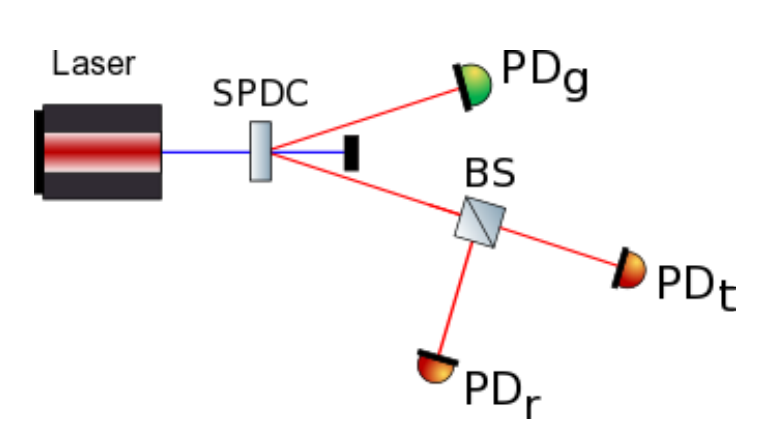
\includegraphics[width = 0.9\textwidth]{../images/our_setup.png}
            \caption{Actual setup}
            \label{our}
        \end{subfigure}

        \begin{subfigure}{\textwidth}
            \centering
            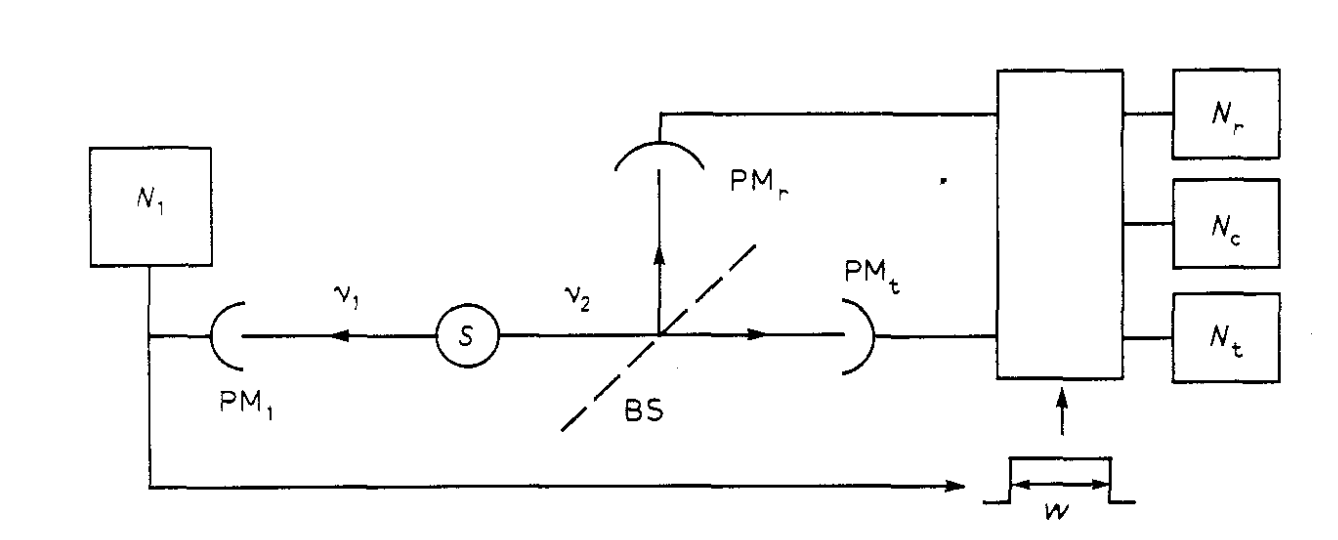
\includegraphics[width = \textwidth]{../images/original.png}
            \caption{Original setup}
        \end{subfigure}
        \caption{Experimental setup scheme}
    \end{figure}
\end{mdframed}
For every gate event which is associated with at least an event in the reflected or transmitted channel (and therefore can be considered as an event not belonging to noise of the gate detector), there is a constant probability $p_r$ and $p_t$ to have an event in these channel.

In fact, we can define two Bernoulli random variables $X_r \sim B(p_r)$ and $X_t \sim B(p_t)$ which represents the result of measurement associated with each gate event. In this sense all the data collected can be represented as a stochastic process of i.i.d. variables. Each measurement will be called a \emph{double} coincidence if only one of the two realizations is $1$, and \emph{triple} coincidence if they are both $1$. 

The physical problem is addressed by observing the correlation between the random variables, using the following definition of correlation coefficient: 
\begin{equation*}
    \alpha = \frac{p_c}{p_r p_t} = \frac{\E[X_r X_t]}{\E[X_r]\E[X_t]}.
\end{equation*}
If $\alpha > 1$ the variables are \emph{correlated}, and the classical model is confirmed, indeed if $\alpha < 1$ the variables are \emph{anticorrelated}, and the classical model is rejected in favour of the quantum model. This follows naturally from the concept of a photon indivisibility: if the photon can't be splitted we expect to never find triple coincidences.
Needless to say, we can only have an estimate of this parameter from experimental data: this is carried out as usual extracting a sample mean estimate using the following estimator: if $N_1$ is the number of valid gate events,
\begin{equation*}
    \hat{\alpha} = \frac{\hat{p_c}}{\hat{p_r} \hat{p_t}} = \frac{N_1 \sum_{i=1}^{N_1} X_r X_t}{\sum_{i=1}^{N_1} X_r\sum_{i=1}^{N_1} X_t}.
\end{equation*}
Further comments on this estimator will be presented in the interpretation of result section.
\subsection*{Analysis}
As anticipated, before counting double and triple coincidences, a preprocessing step is necessary to remove noise. First of all, we reject events on the same channel which are distanced by less than $3900$ machine time units, or $MTU$ (defined by $1 MTU = 80.955 ps$). In fact, events whose difference in time is less than $\approx 0.315 \mu s$ could be \emph{afterpulses}, artifacts of the detection devices. After this passage the interarrival time of the three channels is plotted in Figure \ref{exps}, from which we can confirm that the light used is of coherent type, as it follows a Poisson arrival statistics.
\begin{mdframed}
    \begin{figure}[H]
        \centering
        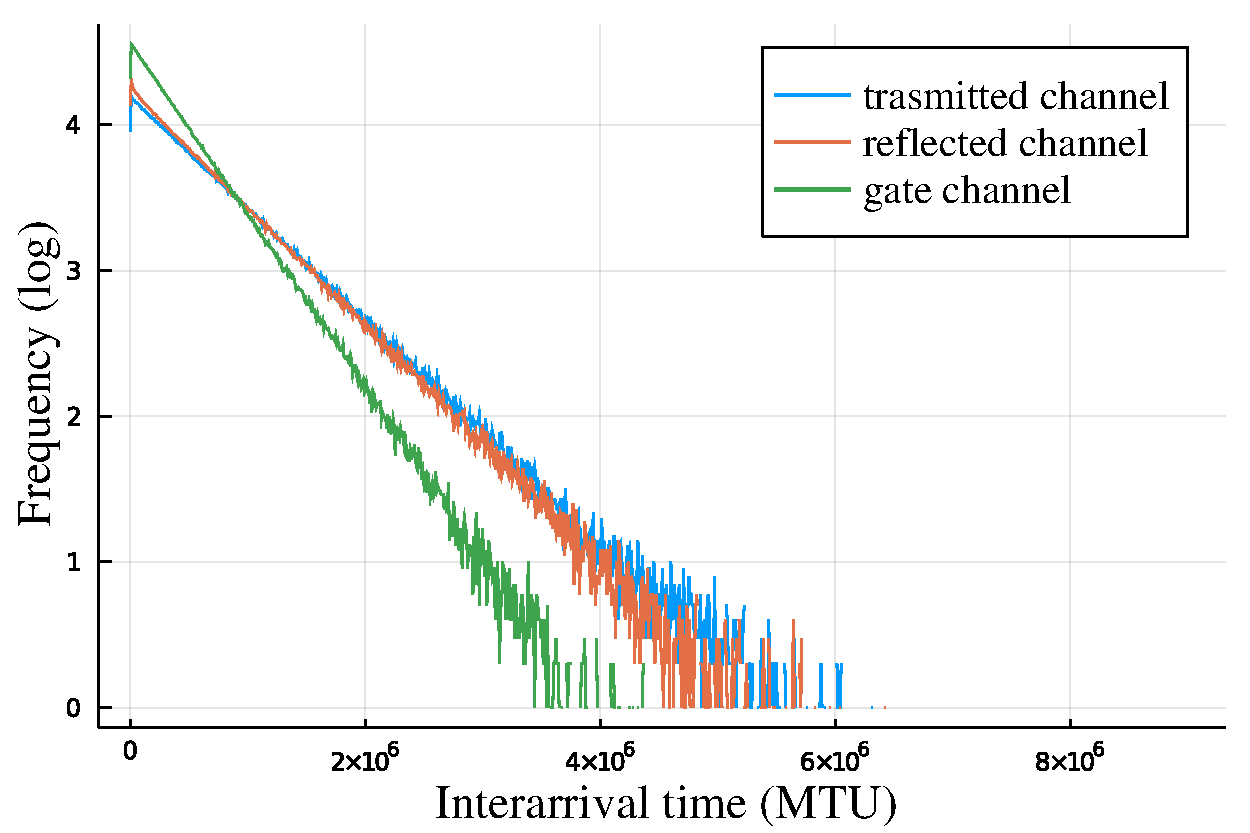
\includegraphics[width = \textwidth]{../images/single_chan.pdf}
        \caption{Single channel click frequencies}
        \label{exps}
    \end{figure}
\end{mdframed}

In a second step, we must filter the data with a suitable \emph{gate} function, which will be triggered by the events on the gate channel, and will detect events from the other channels which are included in a well defined \emph{window}. 

In order to build a correct gate window, we notice that the free air path of photons in the three branches of the optical setup, as well as the difference in the length of the coaxial cables connecting the detector to the time-tagger, can induce a differential time delay of events linked to the same photon pair. So we shall not limit ourselves in looking of equality of time tags as coincidences, as the reflection and/or transmission events related may occur a little time before or after each gate event. By analyzing the total distribution of every channel counts, it will be possible to deduce an estimate of the differential delay of the T and R channels with respect to the nearest gate event.

To facilitate further the recognition of delayed events, we filter the data of the transmitted and reflected channels to be in a strict interval near each gate event.
In general, if we have two photons belonging to the same pair, the differential delay of two detections, on an arbitrary couple of detectors, must be less that a given time. This can be said for \emph{physical reasons}: the pulses reach the time-tagger's front end after the propagation of each photon along the optical bench, and of the signal along the RG cable. Considering the order of magnitude of the lenghts in laboratory, we deduce that the maximum time delay must be in the order of $\sim 10 ns$, so we select only events around $\pm 100 MTU$ away from the nearest gate event. The outcome of this filtering is shown in Figure \ref{before} for the interval $[-100, 0]$, which show only noise, and in Figure \ref{after} for the interval $[0, +100]$ in which bell-shaped delay curves indicates the real delayed occurences.
\begin{mdframed}
    \begin{figure}[H]
        \begin{subfigure}{\textwidth}
            \centering
            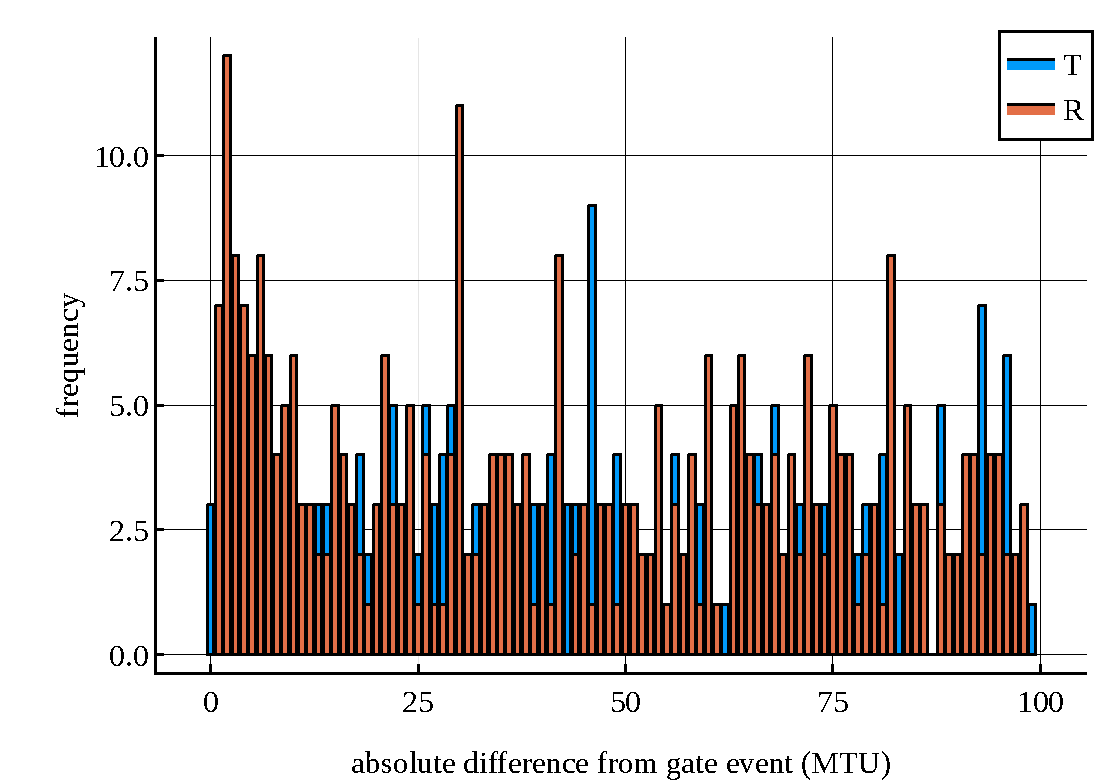
\includegraphics[width = \textwidth]{../images/before.pdf}
            \caption{T, R events before trigger}
            \label{before}
        \end{subfigure}

        \begin{subfigure}{\textwidth}
            \centering
            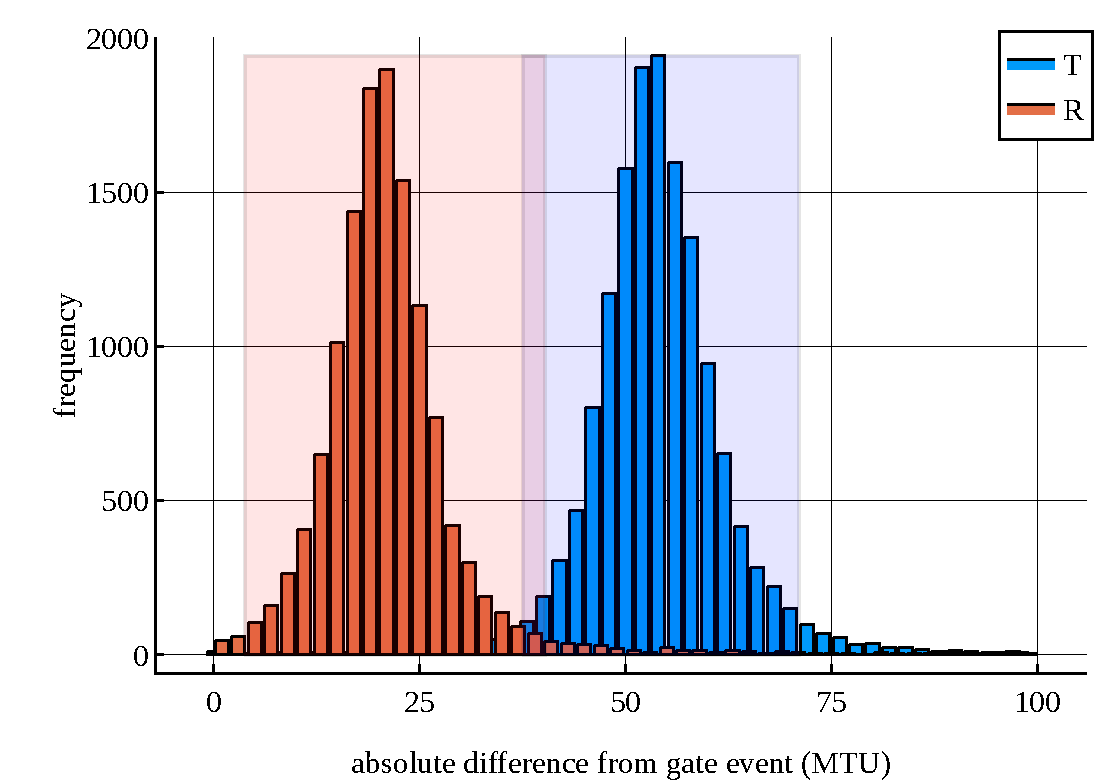
\includegraphics[width = \textwidth]{../images/after.pdf}
            \caption{T, R events after trigger}
            \label{after}
        \end{subfigure}
        \caption{Analysis of inter-channel delay}
    \end{figure}
\end{mdframed}
So we deduce that, in mean, the significant events in the channel R follows the gate event by $\approx 22 MTU$ , and the ones in the T channel follow the gate event by $\approx 54 MTU$.
In conclusion, using the hypotesis that the differential delay follows approximatively  a normal distribution (which can be justified using the Central Limit Theorem), the standard deviations for each bell can be computed using the sample variance, and therefore the \emph{gate} signal is tailored to be a \emph{window} centered in the mean, and of width equal to a desired number of. That windows are shown in Figure \ref{after}, and are of the form $[(t_{Gi} + \mu) -2\sigma; \; (t_{Gi} + \mu) + 2\sigma]$ where $t_{Gi}$ is the time of the $i$-th gate event. Using the $\pm 2 \sigma$ interval, we expect to include in that way the $95\%$ of events. This construction of the gate window considers all the event belonging to the external of the windows as \emph{noise}.  

\subsection*{Interpretation of results}
By filtering the events with the gate function described in the previous paragraph, we are able to measure the realization frequencies associated to the random variables $X_r, \, X_t$. The results are shown in Table \ref{result}, along with estimated errors.
In order to compute the errors, for each probability estimate $\hat{p}$, in the hypotesis of a constant 
\begin{equation}
    \hat{\sigma}_{p} = \frac{\hat{p}(1-\hat{p})}{N_1+1}
\end{equation}
As for the error in $\alpha$, a  should involve its MSE, as the expected value of the error . However, a complete statistical description of this parameter is involved, so a basic error propagation extimate, using Taylor series, is carried out. 
\renewcommand{\arraystretch}{1.5}
\begin{mdframed}
    \begin{table}[H]
        \centering
        \begin{tabular}{|c|c|c|}
            \hline
            $\hat{p}_t (\mathbf{x})$ & $0.4871 \pm 0.003016$\\
            \hline
            $\hat{p}_r (\mathbf{x})$ & $0.5130 \pm 0.003016$\\
            \hline
            $\hat{p}_c (\mathbf{x})$ & $3.6429 \pm 3.6429 \cdot 10^{-5}$\\
            \hline
            $\hat{\alpha} (\mathbf{x})$ & $1.458  \pm 1.4756 \cdot 10^{-4}$\\
            \hline
        \end{tabular}
        \caption{Results}
        \label{result}
    \end{table}
\end{mdframed}
It may seem strange that the estimated errors on $\hat{p}_c$ and $\hat{\alpha}$ are so large to be equal to the actual magnitudes, but this is due to the poor statistics of the sample of triple coincidences: in fact, only 1 over 27451 gate events leads to a triple coincidence, and this greatly compromises the accuracy of the probability estimations. Nonetheless this great uncertainty \emph{does not invalidate the physical conclusions}: this value of $\alpha$ shows a near-perfect anticorrelation, and is complete contradiction whith respect to the classical theory. 

In addition, the result seems to be compatible to the far left part of the ones obtained by Grangier et. al.
\begin{mdframed}
    \begin{figure}[H]
        \centering
        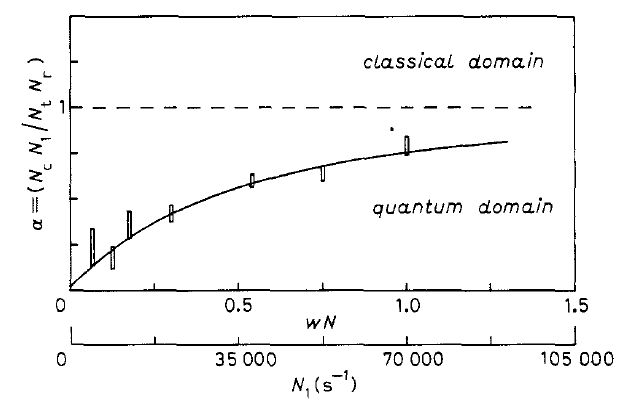
\includegraphics[width = \textwidth]{../images/alpha.png}
        \caption{Original experiment results}
        \label{alpha}
    \end{figure}
\end{mdframed}
So the aim of the experiment is met: this experiment validate the indivisibility of the photons, and, in spite of the classical theory of EM fields, it shows a peculiar quantistic feature of reality. 

\section{Random Number Generation}
In this report two methods of obtaining streams of random bits (i.e. 
 processes of independent and identically distributed Bernoulli $(p = 0.5)$ random variables) are presented.
 Starting from a coherent source of light, the photon arrival times are collected by a time-tagger, so the difference between the arrivals tags represents a realization of a process of exponential random variables. 
 The two methods differ mainly in the fact that their algorithms needs different resources: the first one can operate directly on a continuous stream of photon arrivals, whereas the second needs to scan all the sequence of arrivals before generating, in a second scan, the random bits. We will call the first one \emph{Local difference} method, and the second \emph{Median}, for reasons that will be clear soon.
\subsection*{Local difference method}
This algorithm can operate with constant memory over a stream of subsequent time tags, and works as follows:
\begin{enumerate}
    \item generate from the time tags the vector of the differences between each one with the previous one (skip the first tag), 
    \item select 4 subsequent differences and group them by pairs [(1, 2); (3, 4)], and compute the difference between the second element of the pair and the first one: a sequence $(\Delta_1$, $\Delta_2)$ of 2 values is obtained,
    \item compare the values: if $\Delta_1 \geq \Delta_2$ set the bit to 1, otherwise set the bit to 0, 
    \item iterate 2. to 3. over all the other subsequent group of 8 time tags, and save the deduced bits.
\end{enumerate}
Using the vector of 4353849 time tags belonging to the Arecchi wheel experiment, we generate $4353849/4*8 = 136057$ bytes which represents numbers from 0 to 255. Using them as triplets of coordinates it is possible to build a 3D scatter plot to show their uniform distribution among space. In Figure \ref{local} this representation is shown as well as the histogram of frequencies of numbers.
\begin{mdframed}
    \begin{figure}[H]
        \begin{subfigure}{\textwidth}
            \centering
            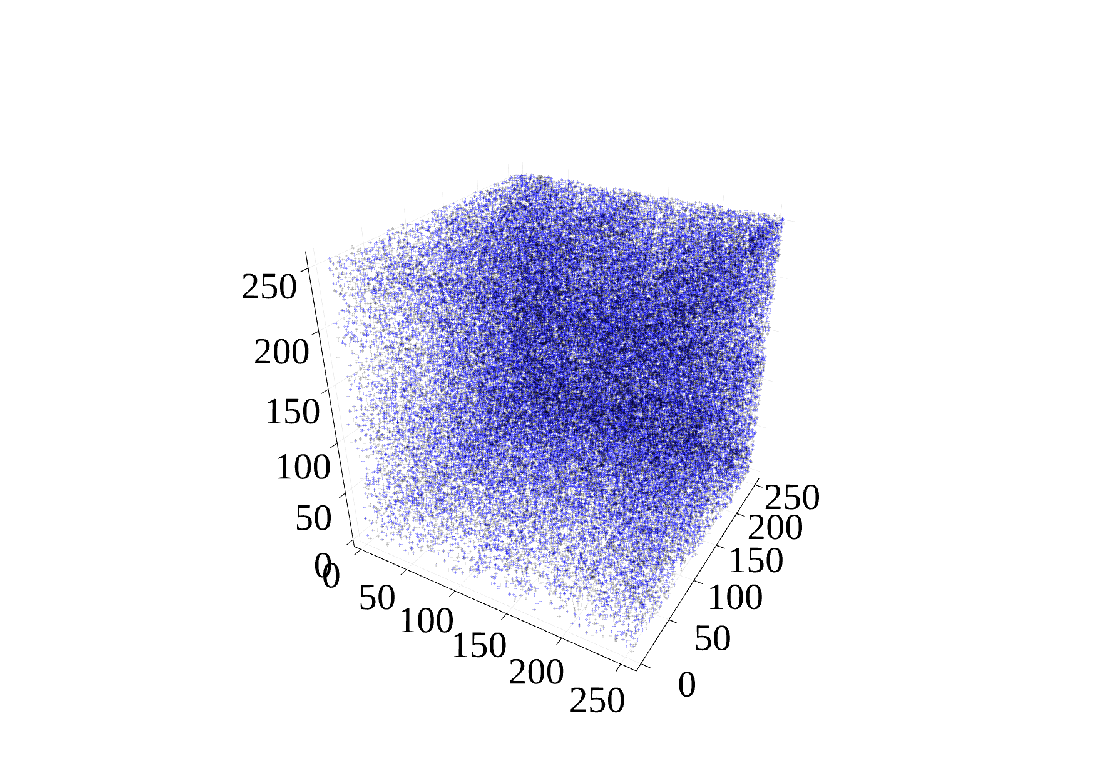
\includegraphics[width = \textwidth]{../random_img/d2-scatter3d.pdf}
            \caption{Scatter 3D}
        \end{subfigure}

        \begin{subfigure}{\textwidth}
            \centering
            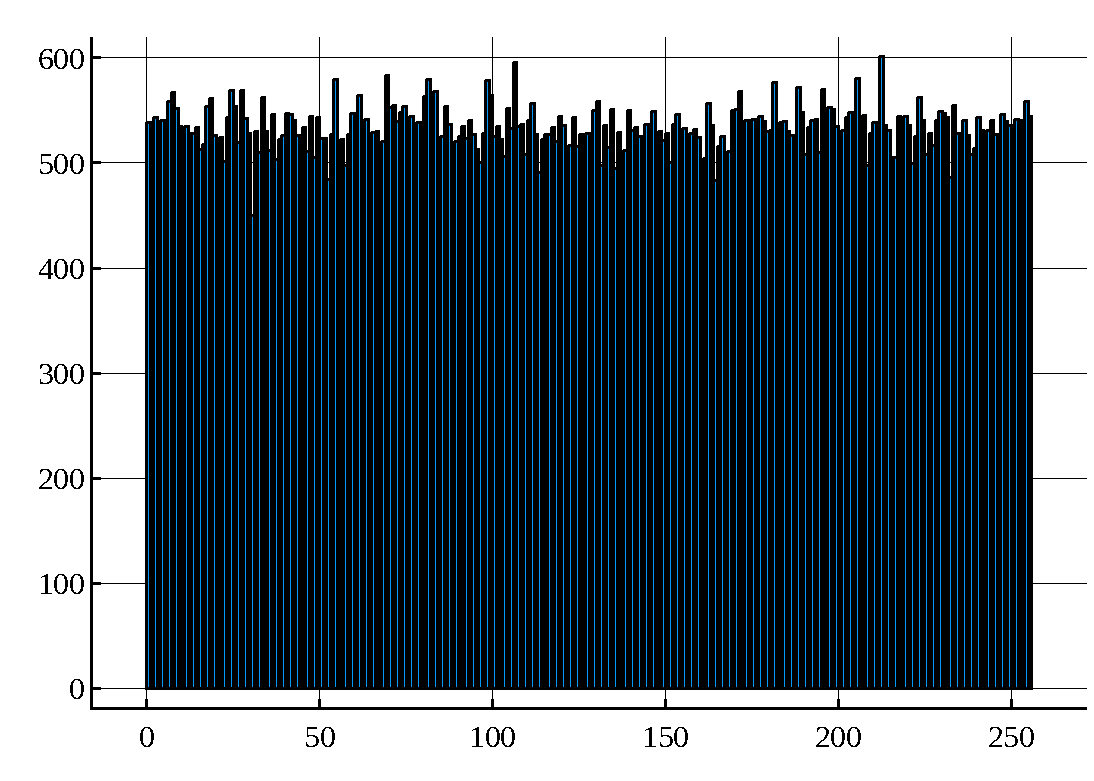
\includegraphics[width = \textwidth]{../random_img/d2-histogram.pdf}
            \caption{Histogram}
        \end{subfigure}
        \caption{Local difference method}
        \label{local}
    \end{figure}
\end{mdframed}

\subsection*{Median method}
This algorithm can operate with a double examination of the stream of the time tags, and works as follows:
\begin{enumerate}
    \item generate from the time tags the vector of the differences between each one with the previous one (skip the first tag),
    \item compute the sample median $\widetilde{d}$ of the differences vector (or alternatively, assuming an exponential distribution, compute the sample mean and obtain the median multiplying it by $ln(2)$),
    \item for each differences sample $d_i$, set a bit to 1 if $d_i \geq \widetilde{d}$, otherwise set it to 0.
\end{enumerate}
This algorithm provides a generation rate of 4 times the Local difference method, at the expense of a greater computing effort, as can be noticed by the plots in Figure \ref{median}.
\begin{mdframed}
    \begin{figure}[H]
        \begin{subfigure}{\textwidth}
            \centering
            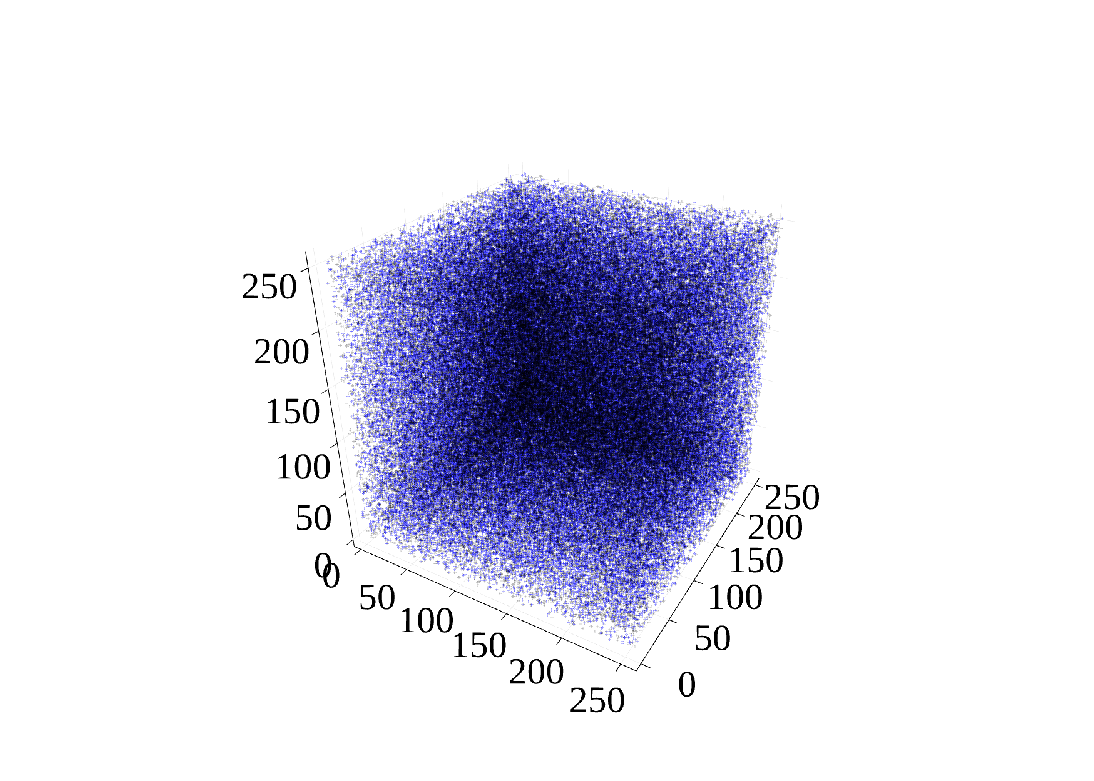
\includegraphics[width = \textwidth]{../random_img/naif-scatter3d.pdf}
            \caption{Scatter 3D}
        \end{subfigure}

        \begin{subfigure}{\textwidth}
            \centering
            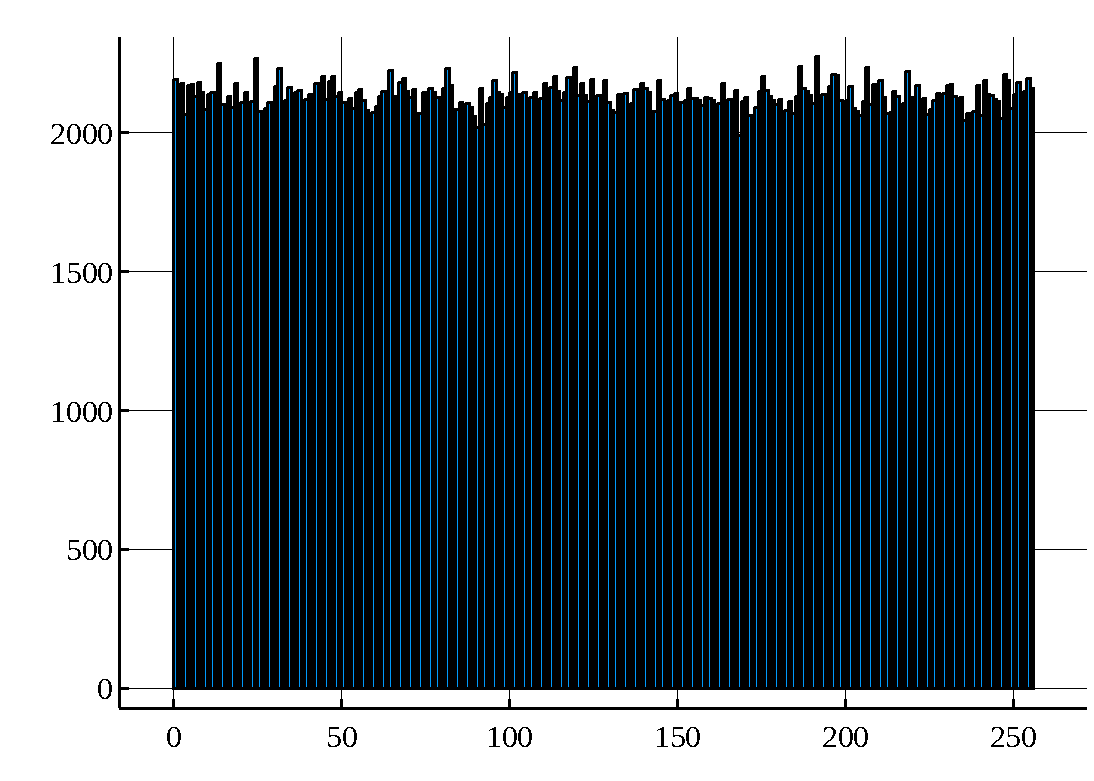
\includegraphics[width = \textwidth]{../random_img/naif-histogram.pdf}
            \caption{Histogram}
        \end{subfigure}
        \caption{Median method}
        \label{median}
    \end{figure}
\end{mdframed}


\subsection*{An even higher bit-rate proposal}
If a complete statistical description of the Poisson arrival process is provided (or estimated observing the dataset), a much higher bit-rate method is easily developed:
We use the theorem of \emph{Universality of uniform r.v.} to obtain a continuous Uniform r.v. $\sim U([0, 1])$ from the Exponential. Once we have obtained that, we can divide the interval $[0, 1]$ in, for example, $256$ sections, and consider for each hit in that section, the corresponding $8$-bit number. The efficiency in this way can be scaled of a factor of $8$ or higher, keeping in mind that the time-tagger has not infinite resolution, and saves the events in a fundamentally discrete space of time tags.
The obvious problem in this method is that the statistical description of the incoming process can only be estimated, so the random bits will be unreliable.


\bibliography{References}
\begin{thebibliography}{99}
  \bibitem{grangier} Grangier, Roger, Aspect
  \bibitem{hc} Hogg Craig, Introduction to mathematical statistics
\end{thebibliography}
\end{multicols}




\hrulefill
\subsection*{Code}

\renewcommand{\baselinestretch}{0.5}
\begin{mdframed}
  \begin{lstlisting}
    module Analyzer
using Plots
using Printf
import Plotly
import PGFPlots
import Statistics
import ProgressMeter

export delay_estimator, main, loader, difference_info, gated_counter, single_chan_stat

Plots.gr()
default(show = true)
# PyPlot.clf()
# println(PyPlot.backend)
const machine_time = 80.955e-12

function loader(;aft_filter = true)
    println("Loading...")
    s = "./tags.txt"
    a = readlines(s)
    for y in a
        filter(x -> !isspace(x), y)
    end
    i=0
    b = Array{Int, 2}(undef, 2, length(a))

    b[1, :] = [parse(Int, split(x, ";")[1]) for x in a]
    b[2, :] = [parse(Int, split(x, ";")[2]) for x in a]


    tags = Array{Int, 2}(undef, 3, length(b))
    fill!(tags, 0)
    println(typeof(tags))
    k = Array{Int, 1}(undef, 3) # k[i] will be the total count of trigger events on channel i
    fill!(k, 1)
    i=0
    cnt = 0
    aft = Array{Int, 1}(undef, 3)
    fill!(aft, 0)
    if (aft_filter)
        aft_const = 3900
    else
        aft_const = 0
    end
    for i = 1:length(a)
         if (i<8 || tags[ b[2, i]-1, k[b[2, i]-1] - 1 ] + aft_const < b[1, i] )
            tags[ b[2, i]-1, k[b[2, i]-1] ] = b[1, i]
            k[b[2, i] - 1] += 1
        else
            # println("Afterpulse on CH-", b[2, i] - 1)
            aft[b[2, i] - 1] +=1
        end
    end

    println("Number of valid hits")
    @printf("\t n. of transmitted hits   : %6d \n", k[1])
    @printf("\t n. of reflected hits     : %6d \n", k[2])
    @printf("\t n. of gate hits          : %6d \n", k[3])
    println("T+R = ", k[1]+k[2], ", G = ", k[3])
    println("Number of afterpulses:")
    @printf("\t chan 1 - transmitted (2) : %6d \n", aft[1])
    @printf("\t chan 2 - reflected (3)   : %6d \n", aft[2])
    @printf("\t chan 3 - gate (4)        : %6d \n", aft[3])
    println("Percentage of afterpulses")
    @printf("\t chan 1 - transmitted (2) : %4.1f %% \n", aft[1]/k[1] * 100)
    @printf("\t chan 2 - reflected (3)   : %4.1f %% \n", aft[2]/k[2] * 100)
    @printf("\t chan 3 - gate (4)        : %4.1f %% \n", aft[3]/k[3] * 100)
    return (tags, k);
end

function delay_estimator((tags, k); mode = "gate_first")
    println("Analyzing...")
    machine_time = 80.955e-12
    diff1 = Array{Int, 1}(undef, k[1])
    diff2 = Array{Int, 1}(undef, k[2])
    fill!(diff1, 0)
    fill!(diff2, 0)
    if mode == "gate_last"
        g1 = -1         # BE CAREFUL : NOT A REAL GATE EVENT
        g2 = tags[3, 1]
        n = 1
        # Retarded gate method - positive diff
        for i = 2:k[3]
            while (tags[1, n]<g2 && n<k[1])
                diff1[n] = g2 - tags[1, n]
                n += 1
            end
            g2 = tags[3, i]
        end

        g1 = -1         # BE CAREFUL : NOT A REAL GATE EVENT
        g2 = tags[3, 1]
        n = 1
        for i = 2:k[3]
            while (tags[2, n]<g2 && n<k[2])
                diff2[n] = g2 - tags[2, n]
                n += 1
            end
            g2 = tags[3, i]
        end
    elseif mode == "gate_first"
        # Anticipated gate method - positive diff
        g1 = -1         # BE CAREFUL : NOT A REAL GATE EVENT
        g2 = tags[3, 1]
        n = 8
        for i = 2:k[3]
            while (tags[1, n]<g2 && n<k[1])
                diff1[n] = tags[1, n] - g1
                n += 1
            end
            g1 = g2
            g2 = tags[3, i]
        end
        diff1 = diff1[8:length(diff1)]

        g1 = -1         # BE CAREFUL : NOT A REAL GATE EVENT
        g2 = tags[3, 1]
        n = 8
        for i = 2:k[3]
            while (tags[2, n]<g2 && n<k[1])
                diff2[n] = tags[2, n] - g1
                n += 1
            end
            g1 = g2
            g2 = tags[3, i]
        end
        diff2 = diff2[8:length(diff2)]
    else
        # Minimum distance method
        g1 = -100000000         # BE CAREFUL : NOT A REAL GATE EVENT
        g2 = tags[3, 1]
        n = 1
        for i = 2:k[3]
            while (tags[1, n]<g2 && n<k[1])
                if ((tags[1, n] - g1) <  (g2 - tags[1, n]))
                    diff1[n] = tags[1, n] - g1
                else
                    diff1[n] = tags[1, n] - g2
                end
                n += 1
            end
            g1 = g2
            g2 = tags[3, i]
        end
        g1 = -100000000         # BE CAREFUL : NOT A REAL GATE EVENT
        g2 = tags[3, 1]
        n = 1
        for i = 2:k[3]
            while (tags[2, n]<g2 && n<k[1])
                if ((tags[2, n] - g1) <  (g2 - tags[2, n]))
                    diff2[n] = tags[2, n] - g1
                else
                    diff2[n] = tags[2, n] - g2
                end
                n += 1
            end
            g1 = g2
            g2 = tags[3, i]
        end
    end

    # max_delay = 7.5 # [ns]
    # max_clicks = max_delay * 1e-9/machine_time
    max_clicks = 80
    max_delay = max_clicks * machine_time / 1e-9
    @printf("PRE-filtering at max delay = %d ns \n ", max_delay)
    # unreal difference filter
    filter!(x-> (x< max_clicks), diff1)
    filter!(x-> (x< max_clicks), diff2)

    filter!(x -> (x>0), diff2)

    difference_info(diff1, diff2, k)
    μ1 = Statistics.mean(diff1)
    μ2 = Statistics.mean(diff2)
    σ1 = sqrt(Statistics.var(diff1 .- μ1))
    σ2 = sqrt(Statistics.var(diff2 .- μ2)) 

    return [μ1, σ1, μ2, σ2]
end

function single_chan_stat((tags, k); chan = 3)
    machine_time = 80.955e-12
    series = tags[chan, :]
    diff = Array{Int, 1}(undef, length(series)-1)
    for i = 1:length(series)-1
        diff[i] = series[i+1] - series[i]
    end
    filter!(z -> (z>0), diff)
    max_diff = maximum(diff)
    println("min: ", minimum(diff))
    bin_num = 1000

    bin_step =Int(ceil(max_diff / bin_num))+1
    println("max diff : ", max_diff, " bin step", bin_step)
    hist = Array{Int, 1}(undef, bin_num)
    fill!(hist, 0)
    i = 1
    for i = 1:length(diff)
        hist[Int(floor((diff[i]) / bin_step)) + 1] += 1
    end
    @printf("minimum difference between gate event: %10d clicks -> %5.2f ns \n",minimum(diff) , minimum(diff)*machine_time/1e-9
    )

    prob = hist / sum(hist)
    accum = 0
    i = 1
    for i = 1:bin_num
        accum += (i-1) * prob[i]
    end
    mu = accum
    var = 0
    sk_acc = 0
    kr_acc = 0 
    for i = 1:bin_num
        var += (i-1 - mu)^2 * prob[i]
        sk_acc += (i-1 - mu)^3 * prob[i]
        kr_acc += (i-1 - mu)^4 * prob[i]
    end
    sigma = sqrt(var)
    sk = sk_acc 
    kr = kr_acc 
    theo_mom = poisson_moments(mu)
    @printf("Statistical analysis of gate events process:\n")
    @printf("\t δ mean                : %5.3f \n", mu  - theo_mom[1])
    @printf("\t δ variance            : %5.3f \n", var - theo_mom[2])
    @printf("\t δ skewness non std    : %5.3f \n", sk  - theo_mom[3])
    @printf("\t δ kurtosis non std    : %5.3f \n", kr  - theo_mom[4])

    fig = Plots.plot((1:bin_num)*bin_step,
                         [log10(h) for h in hist],
                         show=true,
                         xlabel = "absolute difference between gate events (clicks)",
                         size = (1200, 800))
    savefig(fig, string("./images/", chan, "-single_chan.pdf"))
end

function poisson_moments(mu)
    return [mu, mu, 1/sqrt(mu), 1/mu]
end

function bose_ein_moments(mu)
    sigma = sqrt(mu + mu^2)
    return [mu,
            sigma^2,
            (mu + 3*mu^2 + 2*mu^3)/sigma^3,
            (mu + 10*mu^2 + 18*mu^3 + 9*mu^4)/sigma^4]
end

function difference_info(diff1, diff2, k)
    machine_time = 80.955e-12
    println("Difference Info...")
    max_diff1 = maximum(diff1)
    min_diff1 = minimum(diff1)
    max_diff2 = maximum(diff2)
    min_diff2 = minimum(diff2)
    @printf("1) maximum difference      : %10d \n", max_diff1)
    @printf("1) minimum difference      : %10d \n", min_diff1)
    @printf("1) maximum time difference  (ns)  : %10.4f \n", max_diff1 * machine_time * 1e9)
    @printf("1) minimum time difference  (ns)  : %10.4f \n", min_diff1 *machine_time * 1e9)

    @printf("2) maximum difference      : %10d \n", max_diff2)
    @printf("2) minimum difference      : %10d \n", min_diff2)
    @printf("2) maximum time difference  (ns)  : %10.4f \n", max_diff2*machine_time * 1e9)
    @printf("2) minimum time difference  (ns)  : %10.4f \n\n", min_diff2*machine_time * 1e9)

    @printf("1) Fraction of accepted hits : %d / %d = %4.2f \n", length(diff1), k[1], length(diff1)/k[1])
    @printf("2) Fraction of accepted hits : %d / %d = %4.2f\n", length(diff2), k[2], length(diff2)/k[2])

    # Want to show exactly 100 bins in histogram
    mod = Int(ceil(maximum([length(diff1), length(diff2)]) / 1e4)) # TO BE MODIFIED

    # plot clicks 
    x_delays1 = (min_diff1:mod:max_diff1)
    x_delays2 = (min_diff2:mod:max_diff2)

    bin_num1 = Int(floor((max_diff1-min_diff1) / mod)) + 1
    println("bins 1: ", bin_num1)
    bias1 = Int(floor(-min_diff1/mod))
    hist1 = Array{Int, 1}(undef, bin_num1)
    fill!(hist1, 0)
    i = 1
    while (i<=length(diff1))
        hist1[Int(floor((diff1[i] - min_diff1) / mod))+1] += 1
        i += 1
    end

    bin_num2 = Int(floor((max_diff2-min_diff2) / mod)) + 1
    bias2 = Int(floor(-min_diff2/mod))
    println("bins 2: ", bin_num2)
    hist2 = Array{Int, 1}(undef, bin_num2)
    fill!(hist2, 0)
    i = 1
    while (i<=length(diff2))
        hist2[Int(floor((diff2[i] - min_diff2) / mod))+1] += 1
        i += 1
    end
    μ1 = Statistics.mean(diff1)
    μ2 = Statistics.mean(diff2)
    σ1 = sqrt(Statistics.var(diff1 .- μ1))
    σ2 = sqrt(Statistics.var(diff2 .- μ2)) 

    if (length(hist1)<600 && length(hist2)<600)
        println("Plotting...")
        # fig = Plotly.figure()
        n_σ = 2
        fig = Plots.bar(x_delays1,
                         hist1,
                         show=true,
                         title = string("Event delay and ±", n_σ, "σ decision region"),
                         xlabel = "absolute difference from gate event (clicks)",
                         ylabel = "Frequency", 
                         label = "transmitted photon delay", 
                         size = (1000, 600))
        Plots.bar!(x_delays2, hist2, label = "reflected photon delay")
        rectangle(w, h, x, y) = Plots.Shape(x .+ [0,w,w,0], y .+ [0,0,h,h])

        recr = rectangle(2*n_σ*σ1, maximum([maximum(hist1), maximum(hist2)]), μ1-n_σ*σ1, 0)
        rect = rectangle(2*n_σ*σ2, maximum([maximum(hist1), maximum(hist2)]), μ2-n_σ*σ2, 0)
        Plots.plot!(recr, linewidth = 2, opacity = 0.1, color=:blue, label="transmitted decision region")
        Plots.plot!(rect, linewidth = 2, opacity = 0.1, color=:red, label="reflected decision region")

        display(fig)
        savefig("./images/delays.pdf")
    else
        println("Too long to plot...")
    end
end

# need to decide what method to use -> we use  GATE -> REFLECTED -> TRANSMITTED
function gated_counter((tags, k), params; mode = "full-width")
    println("Gated counting...")
    μ1 = params[1]
    σ1 = params[2]
    μ2 = params[3]
    σ2 = params[4]

    @printf("mean reflected   : %6.4f \n", params[1])
    @printf("stdd reflected   : %6.4f \n", params[2])
    @printf("mean tramsmitted : %6.4f \n", params[3])
    @printf("stdd tramsmitted : %6.4f \n", params[4])
    N_1 = length(tags[3, :])
    intervals = [6]
    # Gate function (not counting with multiple hits)
    for n_σ in intervals
        x = 1
        r_hit = false
        refl = 0
        multiple_refl = 0
        y = 1
        t_hit = false
        tran = 0
        multiple_tran = 0
        coincidences = 0
        if (mode == "confidence") 
            for i=1:length(tags[3, :])-1
                r_hit = false
                t_hit = false  
                while  tags[1, x] < -n_σ*σ1 + tags[3, i] + μ1
                    x += 1
                end
                while -n_σ*σ1 + tags[3, i] + μ1 <= tags[1, x] < +n_σ*σ1 + tags[3, i] + μ1 && tags[1, x] < tags[3, i+1] 
                    r_hit = true
                    x += 1
                end
                if r_hit
                    refl += 1
                end

                while  tags[2, y] < -n_σ*σ2 + tags[3, i] + μ2 
                    y += 1
                end
                while -n_σ*σ2 + tags[3, i] + μ2 <= tags[2, y] < +n_σ*σ2 + tags[3, i] + μ2  && tags[2, y] < tags[3, i+1]
                    t_hit = true
                    y += 1
                end
                if t_hit
                    tran += 1
                end
                if r_hit && t_hit
                    coincidences += 1
                end
            end
        else
            for i=1:length(tags[3, :])-1
                r_hit = false
                t_hit = false 
                while tags[1, x] < tags[3, i]
                    x += 1
                end
                while tags[3, i] < tags[1, x] <= tags[3, i+1] 
                    r_hit = true
                    x += 1
                end
                if r_hit
                    refl += 1
                end

                while tags[2, y] < tags[3, i]
                    y += 1
                end
                while tags[3, i] < tags[2, y] <= tags[3, i+1]
                    t_hit = true
                    y += 1
                end
                if t_hit
                    tran += 1
                end
                if r_hit && t_hit
                    coincidences += 1
                end
            end
        end
        @printf("Measurement with ciao confidence \n")
        prob_refl = refl / N_1
        prob_tran = tran / N_1
        prob_triple = coincidences / N_1
        α = prob_triple/ (prob_refl * prob_tran)
        @printf("\t gate         hits :  %9d \n", N_1)
        @printf("\t reflected    hits :  %9d \n", refl)
        @printf("\t transmitted  hits :  %9d \n", tran)
        @printf("\t coincidences hits :  %9d \n", coincidences)
        @printf(" ----------------------\n")
        @printf("\t P[double]         : %9.8f \n", prob_refl + prob_tran)
        @printf("\t P[triple]         : %9.8f \n", prob_triple)
        @printf("\t Alpha             : %9.8f \n", α)
    end
end

function main()
    println("Nothing to do...")
end
end
  \end{lstlisting}
\end{mdframed}

Random number section
\begin{mdframed}
    \begin{lstlisting}
        function random(tags; mode="naif")
        data = diff(tags[1])
        data_diff = diff(data)
        println("Generating with ", mode, " rule...")
        μ =  Statistics.mean(data)
        λ = 1/μ
        median = Statistics.median(data)
        σ = sqrt(Statistics.var(data))
        byte_stream = Array{UInt8}(undef, Int(floor(length(data)/8))-1)
        if mode == "naif"
            stream = BitArray(undef, length(data))
            for i = 1:length(data)
                if data[i]<median
                    stream[i] = 1
                else
                    stream[i] = 0
                end
            end
            byte_stream = Array{UInt8}(undef, Int(floor(length(stream)/8)))
            for i = 1:length(byte_stream)-1
                byte_stream[i] = 1*stream[8*i]+2*stream[8*i+1]+4*stream[8*i+2]+8*stream[8*i+3]+
                                 16*stream[8*i+4]+32*stream[8*i+5]+64*stream[8*i+6]+128*stream[8*i+7]
            end
        elseif mode == "high-rate"
            uniform_events = Array{Float64}(undef, length(data)) 
            for i = 1:length(data)
                uniform_events[i] = exp(-data[i] * λ) - 1
            end
            # fig = Plots.histogram(uniform_events, bin= 10000)
            # display(fig)
            byte_stream = Array{UInt8}(undef, length(data))
            for i = 1:length(byte_stream)
                byte_stream[i] = -Int(floor(255 * uniform_events[i]))
            end
        elseif mode == "diff"
            stream = BitArray(undef, length(data_diff))
            for i =1:length(data_diff)-1
                if data_diff[i]<data_diff[i+1]
                    stream[i] = 1
                else
                    stream[i] = 0
                end
            end
            byte_stream = Array{UInt8}(undef, Int(ceil(length(stream)/8)))
            for i = 1:length(byte_stream)
                byte_stream[i] = 1*stream[8*i]+2*stream[8*i+1]+4*stream[8*i+2]+8*stream[8*i+3]+
                                 16*stream[8*i+4]+32*stream[8*i+5]+64*stream[8*i+6]+128*stream[8*i+7]
            end
        elseif mode == "diff-2"
            stream = BitArray(undef, Int(ceil(length(data))/2))
            fill!(stream, 0)
            k = 1
            for i =1:2:length(data_diff)-2
                if data_diff[i]<data_diff[i+1]
                    stream[k] = 1
                else
                    stream[k] = 0
                end
                k+=1
            end
            byte_stream = Array{UInt8}(undef, Int(ceil(length(stream)/8)))
            fill!(byte_stream, 0)
            for i = 1:length(byte_stream)-8
                byte_stream[i] = 1*stream[8*i]+2*stream[8*i+1]+4*stream[8*i+2]+8*stream[8*i+3]+
                                 16*stream[8*i+4]+32*stream[8*i+5]+64*stream[8*i+6]+128*stream[8*i+7]
            end
        end
        println("Byte stream generated")
        println("mean: ", Statistics.mean(byte_stream))
    
        rnd_tester(byte_stream)
        return byte_stream
    end
    
    function rnd_tester(byte_stream)
        samples = length(byte_stream)-9
        while samples % 3 != 0
            samples -= 1
        end
        println("Analyzing ", samples, " UInt8 numbers...")
        # 3D Scatter
        fig1 = Plots.scatter3d(byte_stream[1:3:samples], byte_stream[2:3:samples], byte_stream[3:3:samples], 
                               markercolor = :blue,
                               markershape = :cross,
                               markersize  = 0.5,
                               opacity = 0.1,
                               label= nothing,
                               tickfont=("times", 12),
                               size = (1024, 768)
                               )  
        # Plots.xaxis!(lims=(0, 255))
        # Plots.yaxis!(lims=(0, 255))
        # Plots.zaxis!(lims=(0, 255))
        # Histogram
        fig2 = Plots.histogram(byte_stream, bins = 256, label= nothing)
        # Random walk
        x = Array{Float64}(undef, samples)
        fill!(x, 0)
        μ = Statistics.mean(byte_stream)
        println("Statistical mean of byte_stream: ", μ)
        for i=2:samples
            x[i] = x[i-1] + byte_stream[i] - μ
        end
        fig3 = Plots.plot(1:samples, x, label= nothing, size = (1024, 768))
    
        display(fig1)
        savefig(fig1, "./random_img/scatter3d.pdf")
        display(fig2)
        savefig(fig2, "./random_img/histogram.pdf")
        display(fig3)
        savefig(fig3, "./random_img/random_walk.pdf")
    end
    \end{lstlisting}
\end{mdframed} 
\end{document}